% Add after the model-configuration results table in Chapter 4.
\begin{figure}[htbp]
\centering
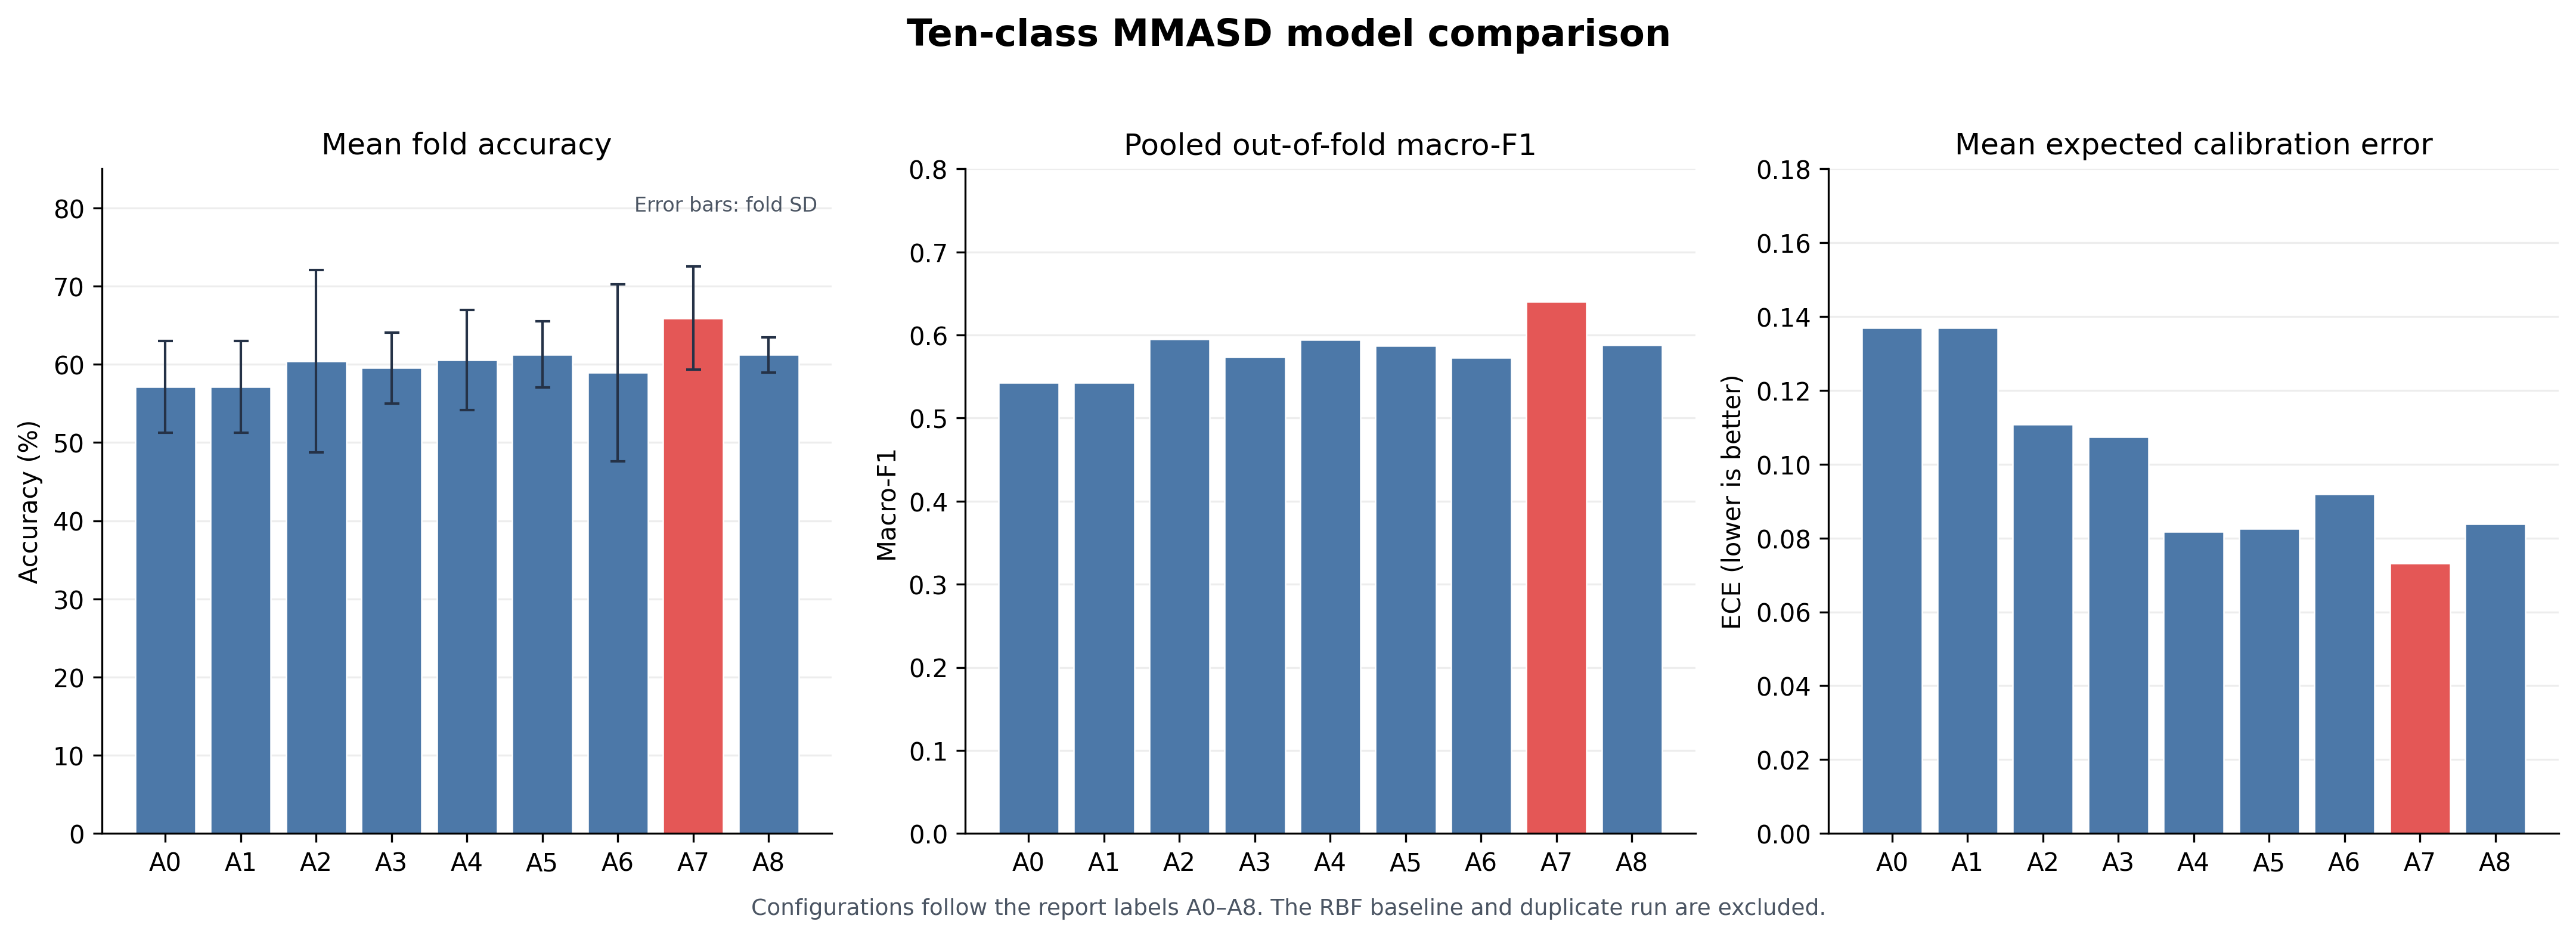
\includegraphics[width=\textwidth]{research_stage4/visualizations/report_ready/ablation_comparison_10class.png}
\caption{Mean fold accuracy, pooled out-of-fold macro-F1, and mean expected calibration error for the distinct tested configurations. Error bars show fold standard deviation for accuracy. The duplicate run and RBF baseline are excluded.}
\label{fig:ablation-comparison}
\end{figure}

% Add after the class-wise F1 table in Chapter 4.
\begin{figure}[htbp]
\centering
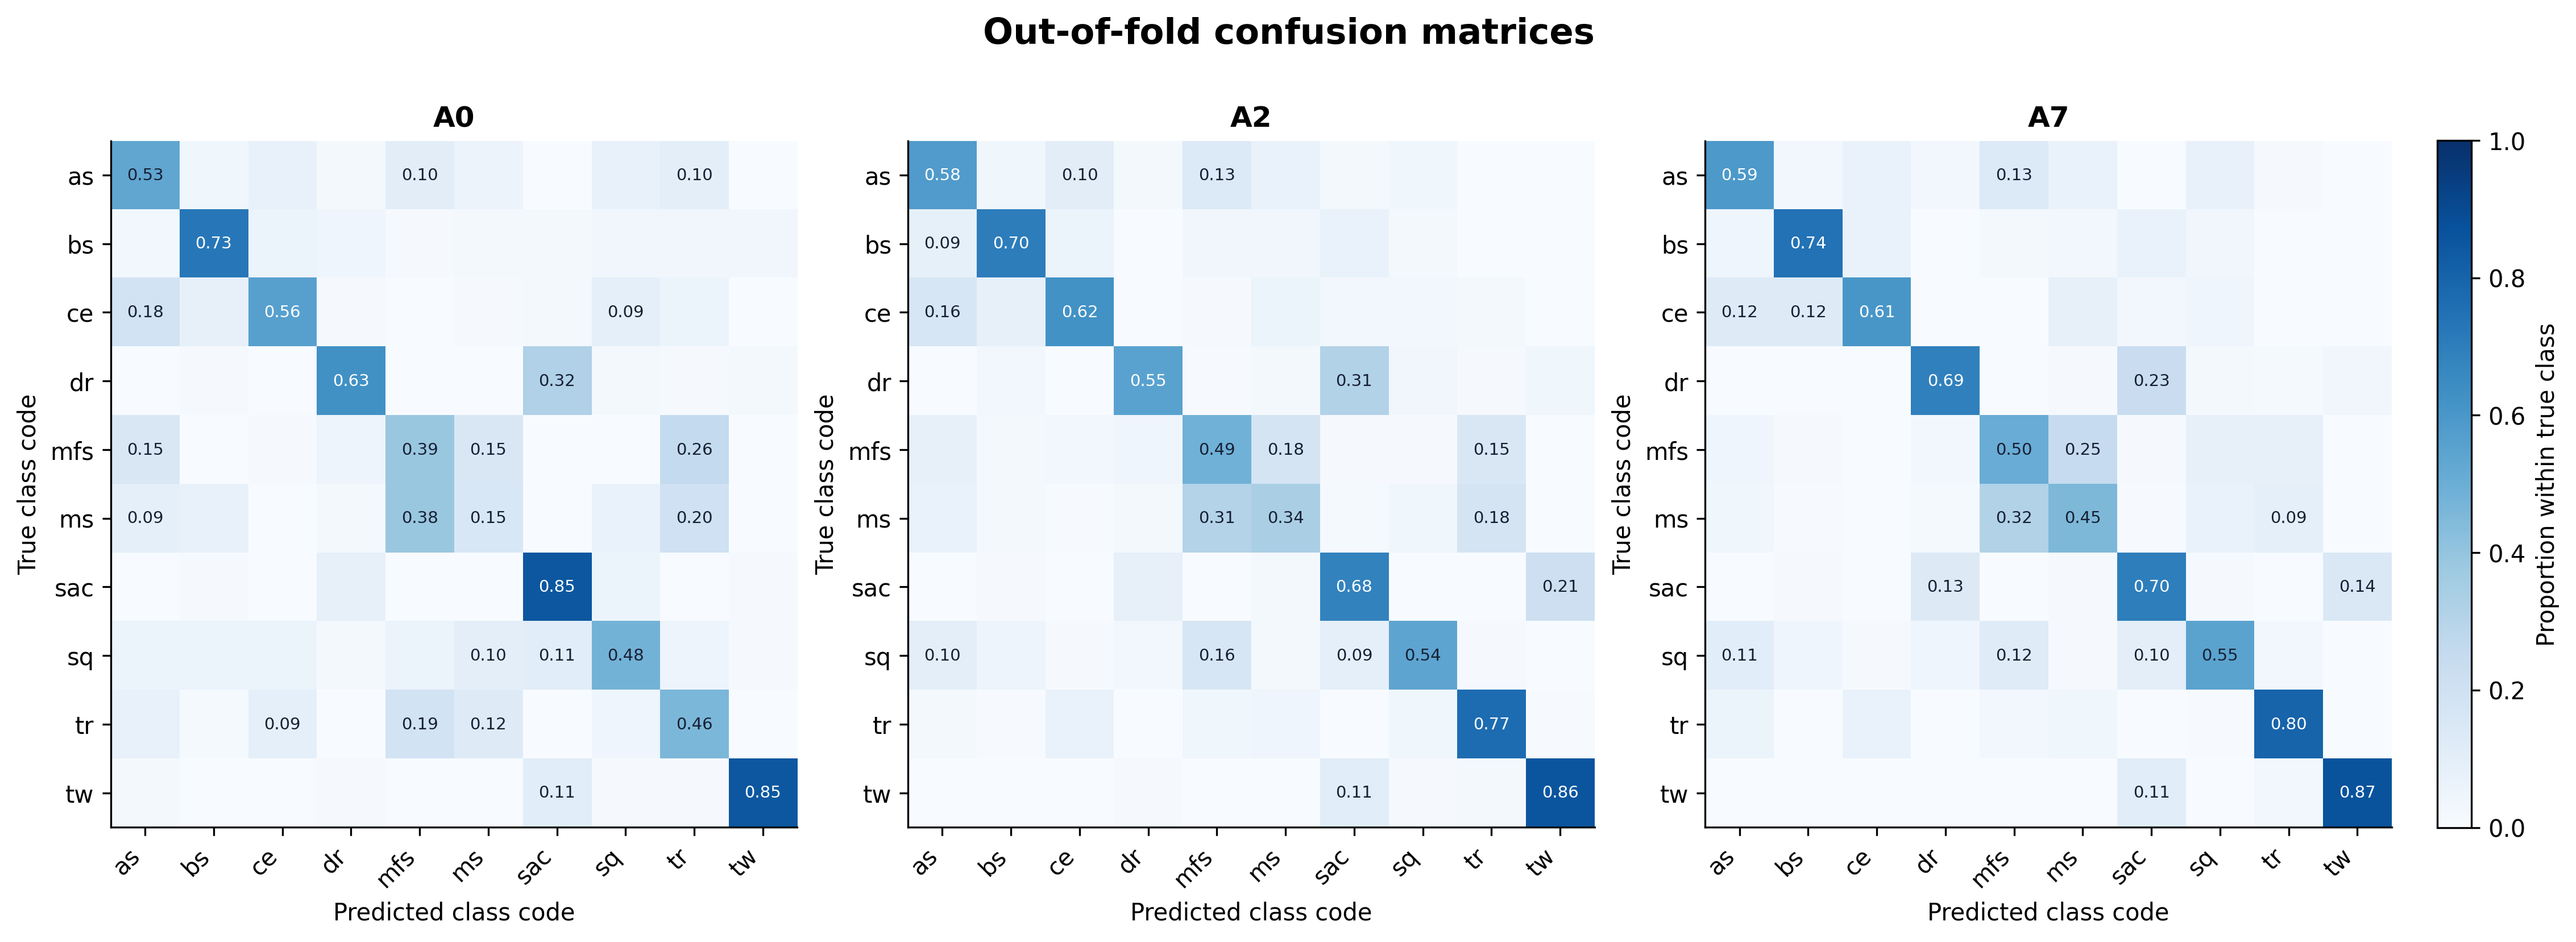
\includegraphics[width=\textwidth]{research_stage4/visualizations/report_ready/confusion_matrices_a0_a2_a7_10class.png}
\caption{Row-normalized out-of-fold confusion matrices for the fixed-connection reference (A0), full RCDB-STGT model (A2), and highest-scoring configuration (A7). Axis labels use the stored MMASD class codes.}
\label{fig:confusion-matrices}
\end{figure}

% Add after the synthetic-corruption results table in Chapter 4.
\begin{figure}[htbp]
\centering
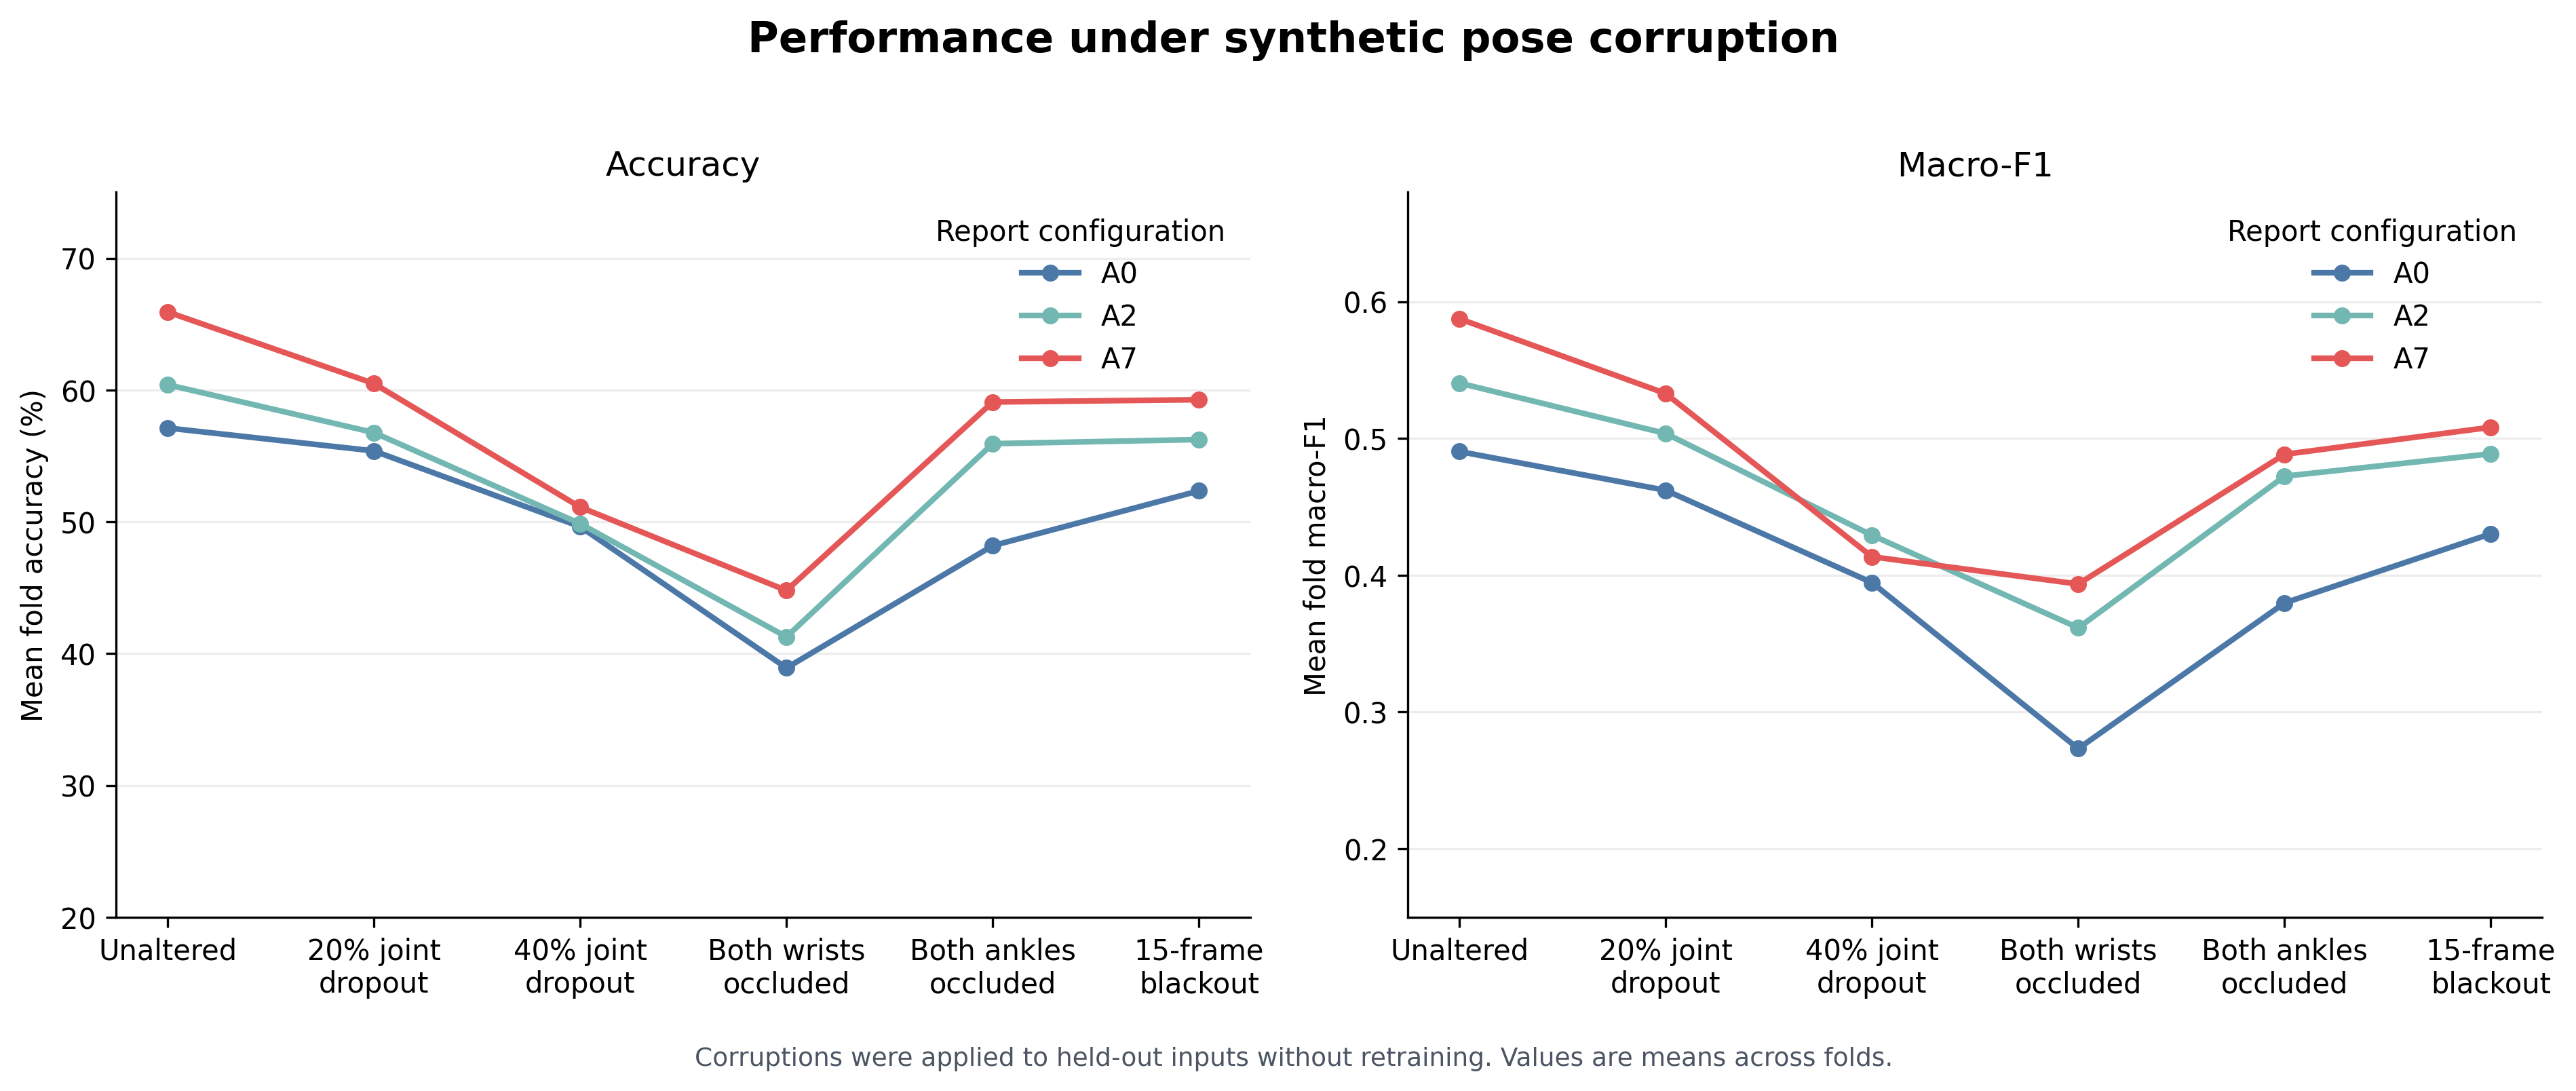
\includegraphics[width=\textwidth]{research_stage4/visualizations/report_ready/synthetic_corruption_comparison_10class.png}
\caption{Accuracy and mean fold macro-F1 under synthetic pose-corruption conditions for A0, A2, and A7. Corruptions were applied to held-out inputs without retraining.}
\label{fig:synthetic-corruption}
\end{figure}

% Optional: add to an appendix or interpretability subsection, not as aggregate performance.
\begin{figure}[htbp]
\centering
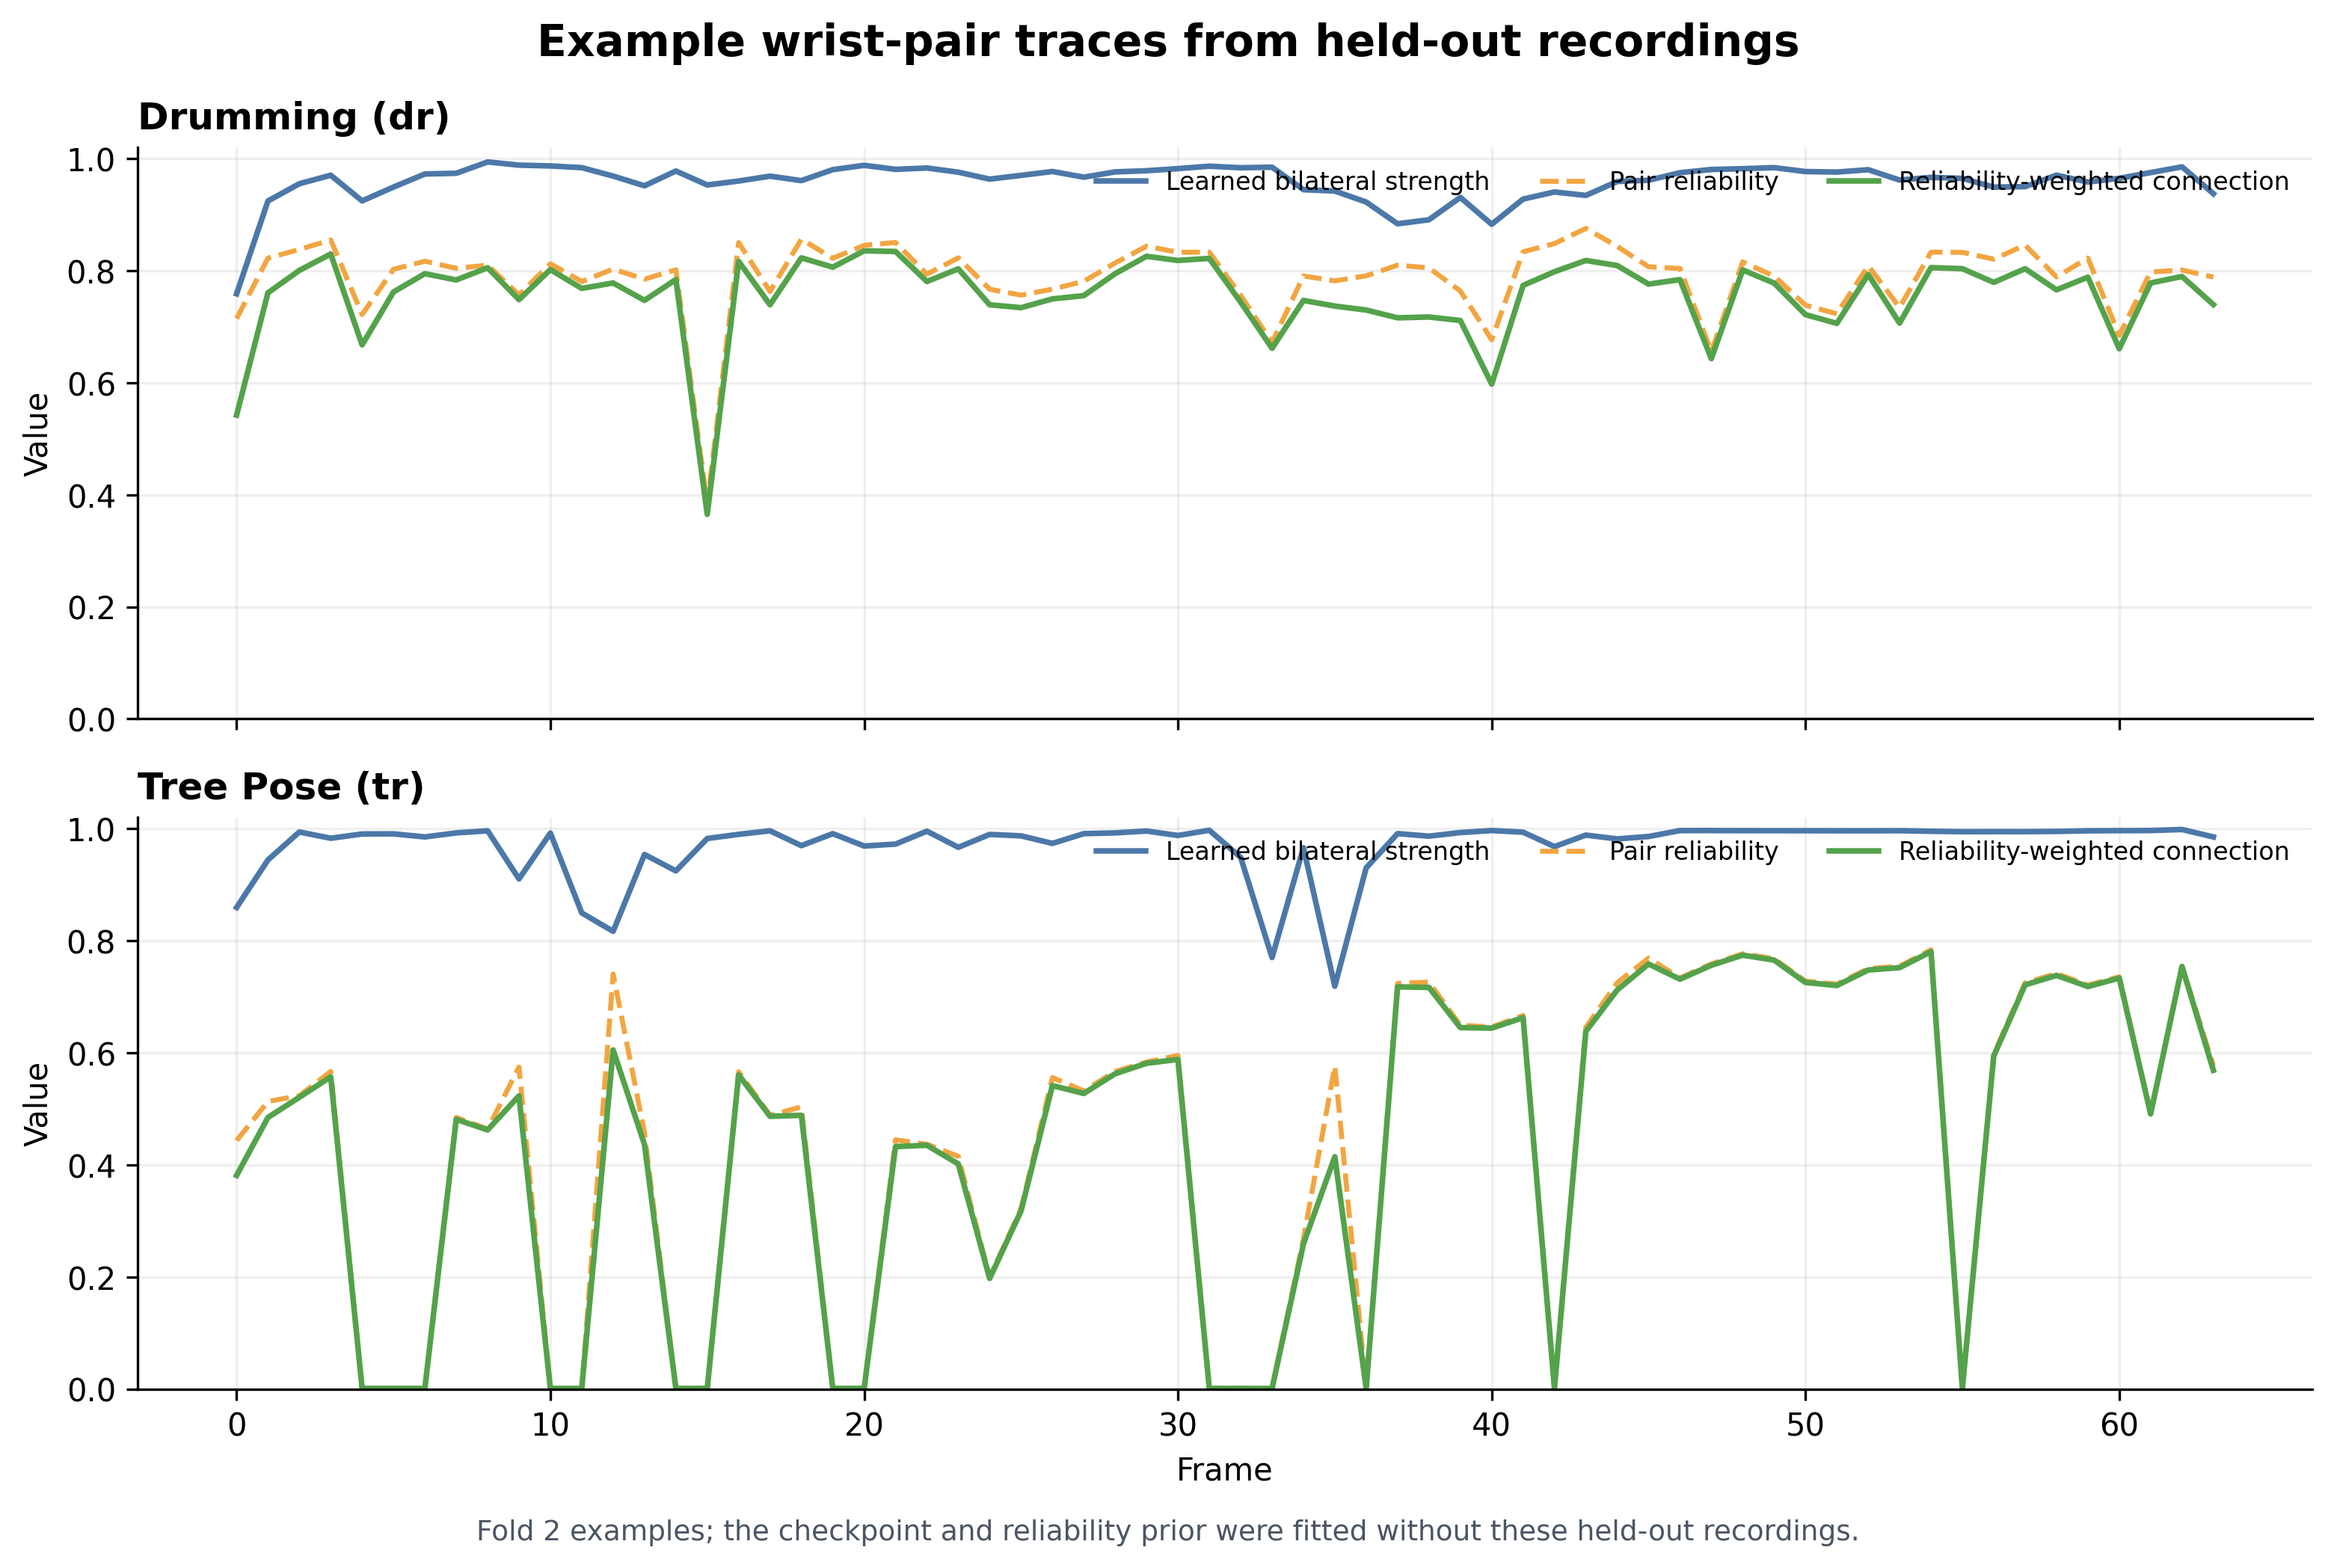
\includegraphics[width=0.9\textwidth]{research_stage4/visualizations/report_ready/bilateral_traces_heldout_fold2.png}
\caption{Illustrative wrist-pair traces for two held-out recordings. The fold-specific checkpoint and reliability prior were fitted without the illustrated recordings. These examples visualize model behavior and are not validated clinical explanations.}
\label{fig:bilateral-traces}
\end{figure}
